\chapter{Query Language}\label{sec:specification_language}

At the heart of the \vnnlib{} standard is the \vnnlib{} query language. Heavily influenced by SMT-LIB, this language is designed as a standardised computer-readable format for expressing a wide range of satisfiability problems over neural networks. This chapter describes the syntax, scoping, typing and semantics of the query language.

\section{Syntax}
\label{sec:syntax}


Similar to SMT-LIB, the syntax of \vnnlib{} is primarily designed with machine-readability in mind. Although the syntax is somewhat human-readable, maximising human-readability is not a primary goal of the language. Instead it is envisaged that \vnnlib{} queries will be generated automatically by higher level tools that provide better human-orientated interfaces.

The syntax of \vnnlib{} is formally defined by the Labelled Backus-Naur Form~\cite{forsberg2005labelled} (LBNF) grammar found in Appendix~\ref{app:lbnf_grammar}. Although we won't describe each of the production rules in detail, we will now describe the key syntactic constructs of the language via illustrative examples.

Firstly, all \vnnlib{} queries are split into two parts: a list of network declarations and a list of assertions. The former allow users to specify an interface for the networks and bring new abstract variables into scope that represent the input and output values of the network. The latter than reference those variables in order to express the desired constraints that should be satisfied. Currently, the standard does not permit the interleaving of network declarations and assertions. Figure~\ref{fig:simple-query} shows an example of a simple query.

\subsection{Simple network declarations}
\label{sec:network-declarations}

 At its simplest, a network is introduced by the keyword \texttt{declare-network}, followed by a user-defined name for the network, and then declarations for its associated input and output. An input is declared using the \texttt{declare-input} keyword, followed by a variable name, its element type (e.g., \texttt{Real}, \texttt{float64}), 
and the shape of the tensor. Similarly, an output variable uses the \texttt{declare-output} keyword. In the case of Figure~\ref{fig:simple-query}, the network is named \texttt{myNetwork}, and it has one input called \texttt{X} consisting of a $1 \times 10$ tensor of real numbers and one output called \texttt{Y} consisting of a $1 \times 2$ tensor of real numbers. 
\begin{figure}[t]
    \begin{minipage}[c]{0.6\textwidth}
        \begin{lstlisting}[style=lbnf]
(declare-network myNetwork
    (declare-input  X Real [1,10])
    (declare-output Y Real [1,2])
)

(assert (>= X[0,2] 0.0))
(assert (<= X[0,2] 1.0))
(assert (<= Y[0,1] 0.5))\end{lstlisting}
    \end{minipage}%
    \begin{minipage}[c]{0.45\textwidth}
        \centering
        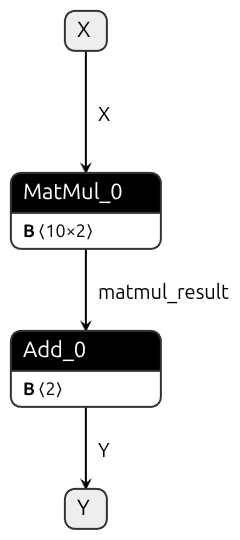
\includegraphics[height=5cm]{imgs/simple_net.onnx.png}
    \end{minipage}
    \caption{A simple \vnnlib{} specification which declares a network with a single input and output. An example of one of the many possible ONNX models compatible with this declaration is shown on the right. Note that the variable names in the declared inputs and outputs do not have to match the node names in the ONNX file.}
    \label{fig:simple-query}
\end{figure}


It is important to clarify that a network declaration only declares an \emph{interface} and by default does not refer in any way to a particular ONNX network model. When passing a query and a network to the verifier, the name of the network does not need to match the name of the ONNX model file. Instead, as described in Section~\ref{sec:verify_command}, the user will explicitly associate a network declaration to the relevant model file via the command line.
Neither do the declared names of the inputs and outputs need to match the names of the input and output nodes within the model file. This flexibility allows many different alternative ONNX models to be compatible with the same query. This also implies that the declared ONNX names of the inputs and outputs, and the network name is not referenced within the Assertions (discussed in Section 3.1.2) of a query.

All variable names follow the same syntax conventions: they are case-sensitive, must start with a letter, and may only contain letters, digits and underscores. All variable names must be unique within the query (see Section~\ref{sec:scoping_and_typing} for a more in-depth discussion). 


% The \texttt{@} character is a reserved character which is used to denote multiple applications of the same network, for the purpose of defining  hyperproperties such as monotonicity. For example \texttt{(declare-network acasXu@1 ...)} and \texttt{(declare-network acasXu@2 ...)} define two networks that are both instances of the same ONNX model,  denoted as \texttt{acasXu} in the command line interface of the verifier (See Chapter~\ref{sec:solver_interface} for more details).

\subsection{Assertions}

The second part of a \vnnlib{} query is a list of assertions that constrain the abstract tensor variables introduced by the network declarations. \vnnlib{} supports quantifier-free logical formulas as \textit{assertions}. Assertions are defined using parenthesized \texttt{(assert\ldots)} expressions, and following an SMT-LIB-like prefix syntax with the 
operator preceding its operands. An assertion is a logical formula that may include logical connectives, relational comparisons, and arithmetic expressions over declared tensors and constants.
The final satisfiability problem is then the conjunction of all the assertions.
 
\paragraph{Constants}

Numeric constant values may be referenced using basic standard integer or floating point syntax (e.g. \inlinevnn{0}, \inlinevnn{0.0}, \inlinevnn{-0.5}). 

\paragraph{Variables} 

Standard indexing notation may be used to refer to a specific element within the tensor variable. For example, Line 6 in Figure~\ref{fig:simple-query} uses \inlinevnn{X[0,2]}, to refer to the value of the element of the input tensor at row~0, column~2. All indices are zero based and currently the number of indices provided must be equal to the number of dimensions of the variable, i.e. partial indexing is not allowed.

\paragraph{Arithmetic expressions}

One forms arithmetic expressions by recursively combining constant and variable values via prefix notation. Currently the following operators are supported:
\begin{itemize}
	\item \inlinevnn{(- a)}: Negation of a term.
    \item \inlinevnn{(+ a b ...)}: Addition of two or more terms. 
    \item \inlinevnn{(* a b ...)}: Multiplication of two or more terms. 
    \item \inlinevnn{(- a b ...)}: Subtraction of two or more terms. Note that subtraction associates to the left, e.g. \inlinevnn{(- 1 2 3 4)} is the same as \inlinevnn{(- (- (- 1 2) 3) 4)} .
\end{itemize}
Arithmetic operations currently only operate over individual tensor elements and cannot be used to operate over multi-dimensional tensors (see Section~\ref{sec:scoping_and_typing} for detailed typing rules).

\paragraph{Comparisons}

The comparison operators \inlinevnn{<=}, \inlinevnn{>=}, \inlinevnn{<}, \inlinevnn{>}, \inlinevnn{=}, \inlinevnn{!=} can be used to compare the values of two arithmetic operations.
For example, \inlinevnn{(<= a b)} returns true if $a$ is less than or equal to $b$.
    
\paragraph{Boolean expressions} 

One forms boolean expressions by recursively combining comparisons via the following supported logical connectives:
\begin{itemize}
    \item \inlinevnn{(and a b ...)}: Conjunction of two or more terms.
    \item \inlinevnn{(or a b ...)}: Disjunction of two or more terms.
\end{itemize}

\subsection{More complex network declarations}
\label{sec:complex-networks-decls}

Although queries usually relate the input of a single network to its output in some way, queries can be far more complex in general. The neural network may have multiple input or output nodes, or the query may refer to intermediate hidden layers of the network or it may relate the behaviour of multiple networks. All of these use cases can be expressed within the query language.

\paragraph{Multiple input and output declarations}

Neural network that take multi-modal input or produce multi-modal output are becoming increasingly common. For example, the network in Figure~\ref{fig:multi-inputs-outputs} shows a model that takes both an image and meta-data about that image as inputs, and outputs both a bounding box around an identified object of interest and a probability distribution over the possible classs that the object belongs to. 

The query language supports such networks by allowing a network declaration to declare an arbitrary number of inputs and outputs. The question is then how is the list of declared inputs and outputs mapped to the list of inputs and outputs nodes in the ONNX model. There are two ways to specify this mapping: 
\begin{itemize}
    \item \textbf{By order:} the default is that declared inputs and outputs are mapped to the ONNX graph's inputs and outputs by matching the order of declaration in the query to the order of declaration in the ONNX model file. This is demonstrated in the top code snippet in Figure~\ref{fig:multi-inputs-outputs}
    \item \textbf{By name:} alternatively, variables can be explicitly mapped using the names of the nodes within the ONNX graph. If this method is used, all input and output variables within that network declaration must be given an explicit ONNX node name. This is demonstrated in the bottom code snippet in Figure~\ref{fig:multi-inputs-outputs}.
\end{itemize}

\begin{figure}[h!]
    \centering
    \begin{lstlisting}[style=lbnf]
(declare-network multi_io_net
    (declare-input  image    Real [1,3,224,224])
    (declare-input  metadata Real [1,10])
    (declare-output bbox     Real [1 4])
    (declare-output logits   Real [1,1000])
)\end{lstlisting}

    \begin{lstlisting}[style=lbnf]
(declare-network multi_io_net
    (declare-input  metadata Real [1,10]        "metadata")
    (declare-input  image    Real [1,3,224,224] "image")
    (declare-output logits   Real [1,1000]      "logits")
    (declare-output bbox     Real [1,4,2]       "bbox")
)\end{lstlisting}

    \vspace{0.5cm}
    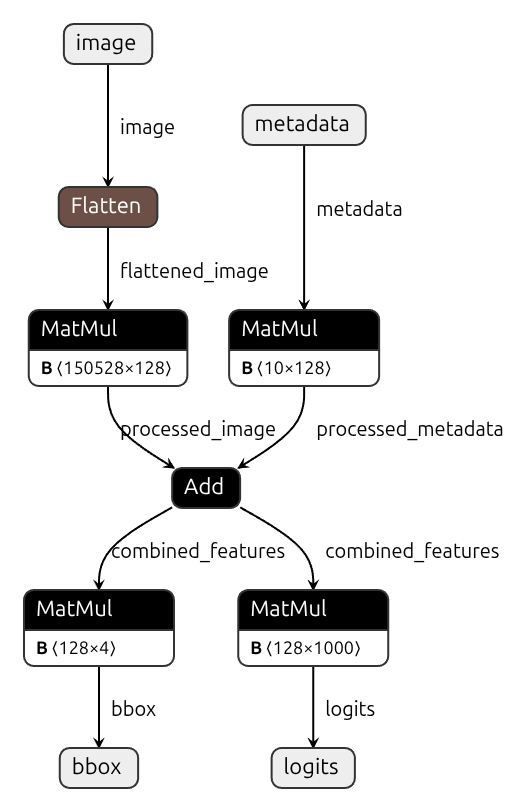
\includegraphics[width=\textwidth]{imgs/multi_io_net.onnx.png}
    \caption{A network with multiple inputs/outputs. The first code snippet shows the declared inputs and outputs mapped to the ONNX inputs and outputs nodes by declaration order, while the second snippet shows them explicitly mapped by the name of the ONNX node.}
    \label{fig:multi-inputs-outputs}
\end{figure}


\paragraph{Hidden output declarations}
\label{sec:hidden-output-declarations}

In some use cases it is desirable to constrain the result of intermediate computation at the output of hidden nodes within the network. For example, when reasoning about the encodings in an encoder-decoder architecture or when reasoning about attention mechanisms. This can be achieved by declaring hidden nodes using the \texttt{declare-hidden} keyword. This declaration includes a variable name for use within the \vnnlib{} specification,  its element type, its tensor shape, and crucially, a string identifier that specifies the corresponding node name in the ONNX graph.  Multiple hidden nodes can be trivially declared within a single network declaration. Figure~\ref{fig:hidden-node} shows a \vnnlib{} network declaration with a hidden node.

The hidden node declaration crucially refers to the uniquely identified outputs of a node, rather than the node (or operator) itself. It declares that an output of the node is to be used as a variable in the \vnnlib{} query.

\begin{figure}[h!]
    \begin{minipage}[c]{0.72\textwidth}
        \begin{lstlisting}[style=lbnf]   
(declare-network encoder
    (declare-input  X Real [1,28,28])
    (declare-hidden Z Real [1,128] "hidden")
    (declare-output Y Real [1,10])
)\end{lstlisting}
    \end{minipage}%
    \begin{minipage}[c]{0.25\textwidth}
        \centering
        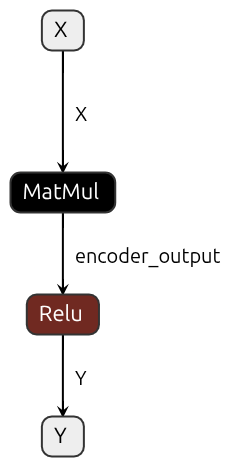
\includegraphics[height=6cm]{imgs/encoder_net.onnx.png}
    \end{minipage}
    \caption{\vnnlib{} network declaration that declares a hidden node}
    \label{fig:hidden-node}
\end{figure}

\paragraph{Multiple networks}

Often you may want to relate the behaviour of one neural network to that of another. Classic examples include: teacher-student networks where you try to train a smaller, more efficient network to mimic the output of the larger network, or observer-controller architectures.

\vnnlib{} supports defining multiple networks in by including multiple \inlinevnn{(declare-network ...)} expressions in the same query. Figure~\ref{fig:multiple-networks} 
shows an example which declares two networks representing a teacher and a student network.

\begin{figure}[h!]
    \begin{minipage}[c]{0.6\textwidth}
        \begin{lstlisting}[style=lbnf]
(declare-network teacher
    (declare-input  tX Real [1,32])
    (declare-output tY Real [1,2])
)

(declare-network student
    (declare-input  sX Real [1,32])
    (declare-output sY Real [1,2])
)\end{lstlisting}
    \end{minipage}
    \begin{minipage}[c]{0.4\textwidth}
        \centering
        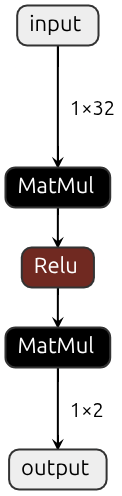
\includegraphics[height=7cm]{imgs/teacher_net.onnx.png}
        \vspace{0.5cm} 
        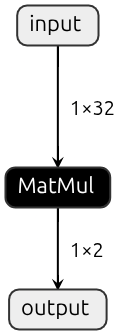
\includegraphics[height=5cm]{imgs/student_net.onnx.png}
    \end{minipage}
    \caption{Two networks declared in \vnnlib{}: \texttt{teacher\_net} and \texttt{student\_net} respectively.}
    \label{fig:multiple-networks}
\end{figure}


\subsection{Comments and whitespace}

Comments in \vnnlib{} are denoted by a semicolon (\texttt{;}) and extend to the end of the line. They are used for annotation, explaining logic, or providing additional context. Whitespace in \vnnlib{} is used to separate tokens and improve readability. It can include spaces, tabs, and newlines. Whitespace is ignored by the parser, except where it is necessary to separate tokens.


\section{Scoping and Typing}
\label{sec:scoping_and_typing}

\subsection{Scoping}
A \vnnlib{} query is said to be \textit{well-scoped}, if it satisfies the following criteria.
\begin{enumerate}
    \item All variables must declared before they are referenced.
    \item All variables are \textit{globally scoped}. All variables are scoped to the entire body of the query.
    \item All variable declarations are \textit{ordered} within network declarations such that inputs before hidden outputs, and hidden outputs before outputs.
    \item All variables have unique names within the query. No variable name is reused within the same query.
\end{enumerate}

\subsection{Typing}
A \vnnlib{} query is said to be \textit{well-typed}, if it satisfies the following criteria.

\begin{itemize}
    \item All variables have a valid ONNX element type.
    \item Variables are \textit{strictly-typed}; so all variable references must match the expected element type in the context where it is substituted.
\end{itemize}
\myremark{
    % Although some ONNX types can be soundly cast for operations in certain cases, for example, a \textit{float16} can be added safely to a \textit{float32} if the expected type of evaluated expression is a \textit{float32}.
    If a query is agnostic to the element type of variables, it should be declared with the \textit{Real} type.
}

\subsubsection*{Typing Rules}

The typing syntax and judgements of a vnnlib{} query is given in  Figure ?. \\
In a \vnnlib{} query, Network Declarations are used to construct the static context ($\Gamma$) which is used to type the variables and literals used in the Assertions of a query.


\begin{figure}
    \centering
    \begin{minipage}[t]{1\textwidth}
        \centering
            \begin{tabular}{@{}lcl@{}}
            $\langle$ElementType$\rangle$ & $\ni$ & 
            \begin{tabular}[t]{@{}l@{}}
                $\tau ::= \left\{\text{int4, int8, int16, int32, int64,}\right.$ \\
                $\quad\quad\quad\text{uint4, uint8, uint16, uint32, uint64,}$ \\
                $\quad\quad\quad\text{float16, float32, float64, bfloat16,} $\\
                $\quad\quad\quad\text{float8e4m3fn, float8e5m2, float4e2m1,}$\\
                $\quad\quad\quad\left.\text{float8e4m3fnuz, float8e5m2fnuz}\right\} $\\
                \end{tabular} \\
            $\langle$TensorShape$\rangle$ & $\ni$ & $s ::= [i_0, ..., i_n] \quad i \in \mathbb{N}$ \\
            $\langle$VariableName$\rangle$ & $\ni$ & $v ::= \texttt{\textasciicircum[A-Za-z][A-Za-z0-9\_]*\$} \quad \text{(regex)}$ \\
            $\langle$InputDeclaration$\rangle$ & $\ni$ & $I::= (\texttt{declareInput}~v~\tau~s$) \\
            $\langle$HiddenDeclaration$\rangle$ & $\ni$ & $H ::= (\texttt{declareHidden}~v~\tau~s$) \\
            $\langle$OutputDeclaration$\rangle$ & $\ni$ & $O ::= (\texttt{declareOutput}~v~\tau~s$) \\
            $\langle$NetworkDeclaration$\rangle$ & $\ni$ & $D ::= (\texttt{declareNetwork}~v~(I_0~...~I_n)^+~(H_0~...~H_n)^*~(O_0~...~O_n)^+$) \\ \\
            $\langle$Double$\rangle$ & $\ni$ & $d ::= \mathbf{Double}$ \\
            $\langle$TensorIndex$\rangle$ & $\ni$ & $j ::= [i_0,...,i_n]^+ \quad i \in \mathbb{N}$ \\
            $\langle$ArithExpr$\rangle$ & $\ni$ & 
                \begin{tabular}[t]{@{}l@{}}
                $a ::= d$ \\
                $\quad\;|\; v~j$ \\
                $\quad\;|\; (\texttt{-}~a$) \\
                $\quad\;|\; (\texttt{+}~a_0~...~a_n$) \\
                $\quad\;|\; (\texttt{×}~a_0~...~a_n$) \\
                $\quad\;|\; (\texttt{-}~a_0~...~a_n$) \\
                \end{tabular} \\
            $\langle$BoolExpr$\rangle$ & $\ni$ & 
                \begin{tabular}[t]{@{}l@{}}
                $b ::= (\texttt{>=}~a_1~a_2$) \\
                $\quad\;|\; (\texttt{>}~~a_1~a_2$) \\
                $\quad\;|\; (\texttt{<=}~a_1~a_2$) \\
                $\quad\;|\; (\texttt{<}~~a_1~a_2$) \\
                $\quad\;|\; (\texttt{==}~a_1~a_2$) \\
                $\quad\;|\; (\texttt{!=}~a_1~a_2$) \\
                $\quad\;|\; (\texttt{and}~b_0~...~b_n$) \\
                $\quad\;|\; (\texttt{or}~b_0~...~b_n$)
                \end{tabular} \\
            $\langle$Assertion$\rangle$ & $\ni$ & $A ::= (\texttt{assert}~b$) \\ \\
            $\langle$Query$\rangle$ & $\ni$ & $Q ::= (D_0~...~D_n)~(A_0~...~A_n)^+$ \\
            \end{tabular}
    \caption{\vnnlib{} format typing syntax}
    \end{minipage}
\end{figure}

\begin{figure}
    \begin{minipage}[t]{1\textwidth}
        \resizebox{\textwidth}{!}{
        \begin{mathpar}
            \inferrule*[Right=InputDeclaration]{\;}{
                \Gamma \vdash (\texttt{declareInput}~v~\tau~s) : \Gamma := \Gamma, v :(\tau,s) 
            }
            \\
            \inferrule*[Right=HiddenDeclaration]{\;}{
                \Gamma \vdash (\texttt{declareHidden}~v~\tau~s) : \Gamma := \Gamma, v :(\tau,s)
            }
            \\
            \inferrule*[Right=OutputDeclaration]{\;}{
                \Gamma \vdash (\texttt{declareOutput}~v~\tau~s) : \Gamma := \Gamma, v :(\tau,s)
            }
            \\
            \inferrule*[Right=NetworkDeclaration]{
                \Gamma_{i=0} := \Gamma \vdash I_0 \\
                \Gamma_{h=0} := \Gamma_I \vdash H_0\\
                \Gamma_{o=0} := \Gamma_H \vdash O_o \\
                \Gamma_{i+1} := \Gamma_i \vdash I_i \\
                \Gamma_{h+1} := \Gamma_h \vdash H_h \\
                \Gamma_{o+1} := \Gamma_o \vdash O_o \\
            }{
                \Gamma \vdash (\texttt{declareNetwork}~v~(I_0~...~I_n)^+~(H_0~...~H_n)^*~(O_0~...~O_n)^+) : \Gamma_O
            } \\
            \hspace*{\fill}\text{\small where $\Gamma_O$ is the final context after extending by the last output declaration}
            \\ \\ \\
            \inferrule*[]{\;}{
                \Gamma \Vdash d : \tau
            }
            \hspace{1cm}
            \inferrule*[]{
                \Gamma [v] : (\tau,s) \quad j : \text{validIndices} (j, s)
            }{
                \Gamma \Vdash v~j : \tau
            }
            \hspace{1cm}
            \inferrule*[Right=ArithExpr]{
                \Gamma \Vdash a : \tau
            }{
                \Gamma \Vdash (\texttt{-}~a) : \tau
            }
            \\
            \inferrule*[Right=ArithExpr N-ary]{
                \Gamma \Vdash a_0 : \tau \quad ... \quad \Gamma \Vdash a_n : \tau
            }{
                \Gamma \Vdash (\circledast~a_0~...~a_n) : \tau \quad \circledast \in \{\texttt{+}, \texttt{-}, \texttt{×}\}
            }
            \\
            \inferrule*[Right=BoolExpr Comparisons]{
                \Gamma \Vdash a_1 : \tau \quad \Gamma \Vdash a_2 : \tau
            }{
                \Gamma \Vdash (\lozenge~a_1~a_2) : \mathbf{Bool} \quad \lozenge \in \{\texttt{>=}, \texttt{>}, \texttt{<}, \texttt{<=}, \texttt{==}, \texttt{!=}\}
            }
            \\
            \hspace{1cm}
            \inferrule*[Right=BoolExpr]{
                \Gamma \Vdash b_0 :  \mathbf{Bool} \quad ... \quad \Gamma \Vdash b_n : \mathbf{Bool}
            }{
                \Gamma \Vdash (\Box~b_0~...~b_n) : \mathbf{Bool} \quad \Box \in \{\texttt{and}, \texttt{or}\}
            }
        \end{mathpar}
        }
    \caption{Typing judgements}
    \end{minipage}
\end{figure}

\section{Semantics}
\label{sec:semantics}

\mnote{TODO: Ann Roy}
